
\documentclass{mcmthesis}
\mcmsetup{CTeX = false,   % 使用 CTeX 套装时,设置为 true
        tcn = 77281, problem = A,
        sheet = true, titleinsheet = true, keywordsinsheet = true,
        titlepage = true, abstract = true}
\usepackage{palatino}

\title{The \LaTeX{} Template for MCM Version \MCMversion}
\date{\today}
\begin{document}
\begin{abstract}

Summary Sheet: The summary is an essential part of your MCM/ICM paper. The judges place considerable weight on the summary, and winning papers are often distinguished from other papers based on the quality of the summary.

To write a good summary, imagine that a reader will choose whether to read the body of the paper based on your summary: Your concise presentation in the summary should inspire a reader to learn about the details of your work. Thus, a summary should clearly describe your approach to the problem and, most prominently, your most important conclusions.  Summaries that are mere restatements of the contest problem, or are a cut-and-paste boilerplate from the Introduction are generally considered to be weak.

Besides the summary sheet as described each paper should contain the following sections:

\begin{itemize}
\item Restatement and clarification of the problem: State in your own words what you are going to do.
\item Explain assumptions and rationale/justification: Emphasize the assumptions that bear on the problem. Clearly list all variables used in your model.
\item Include your model design and justification for type model used or developed.
\item Describe model testing and sensitivity analysis, including error analysis, etc.
\item Discuss the strengths and weaknesses of your model or approach.
\end{itemize}

\begin{keywords}
keyword1; keyword2
\end{keywords}

\end{abstract}
\maketitle
\section{Introduction}


\begin{itemize}
\item minimizes the discomfort to the hands, or
\item maximizes the outgoing velocity of the ball.
\end{itemize}
We focus exclusively on the second definition.

\begin{itemize}
\item the initial velocity and rotation of the ball,
\item the initial velocity and rotation of the bat,
\item the relative position and orientation of the bat and ball, and
\item the force over time that the hitter hands applies on the handle.
\end{itemize}

\begin{itemize}
\item the angular velocity of the bat,
\item the velocity of the ball, and
\item the position of impact along the bat.
\end{itemize}

\emph{center of percussion} [Brody 1986], 

\begin{Theorem} \label{thm:latex} %定理
\LaTeX
\end{Theorem}
\begin{Lemma} \label{thm:tex}  %引理
\TeX .
\end{Lemma}
\begin{proof}
The proof of theorem.
\end{proof}

\subsection{Other Assumptions}  %假设

\begin{itemize}
\item
\item
\item
\item
\end{itemize}


\section{Analysis of the Problem}
\begin{figure}[h]
\small
\centering
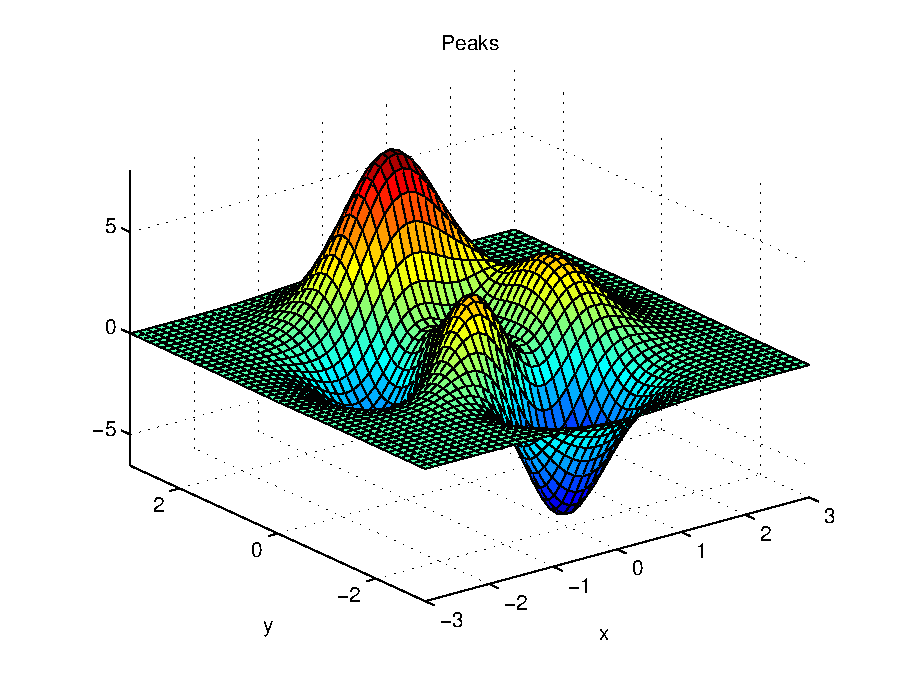
\includegraphics[width=12cm]{mcmthesis-aaa.eps}
\caption{aa} \label{fig:aa}
\end{figure}

\eqref{aa}
\begin{equation}
a^2 \label{aa}
\end{equation}

\[
  \begin{pmatrix}{*{20}c}
  {a_{11} } & {a_{12} } & {a_{13} }  \\
  {a_{21} } & {a_{22} } & {a_{23} }  \\
  {a_{31} } & {a_{32} } & {a_{33} }  \\
  \end{pmatrix}
  = \frac{{Opposite}}{{Hypotenuse}}\cos ^{ - 1} \theta \arcsin \theta
\]


\[
  p_{j}=\begin{cases} 0,&\text{if $j$ is odd}\\
  r!\,(-1)^{j/2},&\text{if $j$ is even}
  \end{cases}
\]



\[
  \arcsin \theta  =
  \mathop{{\int\!\!\!\!\!\int\!\!\!\!\!\int}\mkern-31.2mu
  \bigodot}\limits_\varphi
  {\mathop {\lim }\limits_{x \to \infty } \frac{{n!}}{{r!\left( {n - r}
  \right)!}}} \eqno (1)
\]

\section{Calculating and Simplifying the Model  }

\section{The Model Results}


\section{Validating the Model}


\section{Conclusions}


\section{A Summary}


\section{Evaluate of the Mode}

\section{Strengths and weaknesses}


\subsection{Strengths}
\begin{itemize}
\item \textbf{Applies widely}\\
This  system can be used for many types of airplanes, and it also
solves the interference during  the procedure of the boarding
airplane,as described above we can get to the  optimization
boarding time.We also know that all the service is automate.
\item \textbf{Improve the quality of the airport service}\\
Balancing the cost of the cost and the benefit, it will bring in
more convenient  for airport and passengers.It also saves many
human resources for the airline. 
\item \textbf{}
\end{itemize}

\begin{thebibliography}{99}
\bibitem{1} D.~E. KNUTH   The \TeX{}book  the American
Mathematical Society and Addison-Wesley
Publishing Company , 1984-1986.
\bibitem{2}Lamport, Leslie,  \LaTeX{}: `` A Document Preparation System '',
Addison-Wesley Publishing Company, 1986.
\bibitem{3}\url{http://www.latexstudio.net/}
\bibitem{4}\url{http://www.chinatex.org/}
\end{thebibliography}

\begin{appendices}

\section{First appendix}



Here are simulation programmes we used in our model as follow.\\

\textbf{\textcolor[rgb]{0.98,0.00,0.00}{Input matlab source:}}
\lstinputlisting[language=Matlab]{./code/mcmthesis-matlab1.m}

\section{Second appendix}

some more text \textcolor[rgb]{0.98,0.00,0.00}{\textbf{Input C++ source:}}
\lstinputlisting[language=C++]{./code/mcmthesis-sudoku.cpp}

\end{appendices}
\end{document}

%% 
%% This work consists of these files mcmthesis.dtx,
%%                                   figures/ and
%%                                   code/,
%% and the derived files             mcmthesis.cls,
%%                                   mcmthesis-demo.tex,
%%                                   README,
%%                                   LICENSE,
%%                                   mcmthesis.pdf and
%%                                   mcmthesis-demo.pdf.
%%
%% End of file `mcmthesis-demo.tex'.
